\documentclass[conference]{IEEEtran}
\IEEEoverridecommandlockouts
\usepackage{cite}
\usepackage{amsmath,amssymb,amsfonts}
\usepackage{algorithmic}
\usepackage{graphicx}
\usepackage{textcomp}
\usepackage{xcolor}
\usepackage{multirow}
\usepackage{booktabs}
\usepackage{array}
\usepackage{url}

\def\BibTeX{{\rm B\kern-.05em{\sc i\kern-.025em b}\kern-.08em
    T\kern-.1667em\lower.7ex\hbox{E}\kern-.125emX}}

\begin{document}

\title{GDP (Generative Digital-twin Prototyper): An LLM-Based Framework for Automated Process Design and Analysis Tool Integration}

\author{\IEEEauthorblockN{Geonchang Lee}
\IEEEauthorblockA{\textit{Department of Digital Media and Communications Engineering} \\
\textit{Sunghyunkwan University}\\
Suwon, Republic of Korea \\
ilsc2908@skku.edu}
\and
\IEEEauthorblockN{Honguk Woo\textsuperscript{*}}
\IEEEauthorblockA{\textit{Department of Software} \\
\textit{Sunghyunkwan University}\\
Suwon, Republic of Korea \\
hwoo@skku.edu}
}

\maketitle

\begin{abstract}
Implementing digital twins, a core technology of smart industry, requires sophisticated manufacturing data and a simulation framework built upon it. However, real-world manufacturing faces a dual barrier: data inaccessibility that prevents non-experts from entering the field, and interface fragmentation between tools that burdens experts. In this paper, we propose GDP (Generative Digital-twin Prototyper), a framework that leverages large language models (LLMs) to simultaneously address both user groups. First, GDP enables non-experts and researchers to generate mock process data in a zero-shot manner without manufacturing knowledge, providing a virtual testbed applicable to Physical AI research including humanoid robots. To this end, GDP adopts the Bill of Process (BOP) concept proposed by Siemens for reliable process modeling. Second, GDP dramatically reduces the interface construction cost that experts and developers face when integrating simulation and optimization tools, through LLM-based automatic adapter generation and an Auto-Repair mechanism. Experimental results show that zero-shot process generation across 10 product families achieves an F1 of 88.9\%, demonstrating the feasibility of data acquisition by non-experts. In tool integration experiments for experts, Auto-Repair achieves a 100\% execution pass rate while observing 16.2\% ``silent failures,'' demonstrating the necessity of two-tier evaluation beyond execution-only assessment.
\end{abstract}

\begin{IEEEkeywords}
Digital Twin, LLM, Manufacturing, Bill of Process, Tool Integration, Auto-Repair
\end{IEEEkeywords}

%% ============================================================
\section{Introduction}
%% ============================================================

Manufacturing competitiveness in the era of smart industry hinges on the maturity of digital twin technology that replicates physical factories in virtual space for pre-verification. Digital twins enable bottleneck prediction, process optimization, and real-time monitoring at the design stage, establishing themselves as core infrastructure for manufacturing innovation~\cite{b1}. However, advancing digital twins at the research and development stage faces two major barriers.

The first is the \textbf{absence and fragmentation of benchmark data}. Real manufacturing data is strictly restricted from public disclosure as a core security asset, making it difficult for external researchers to obtain reliable open datasets for simulation advancement.

The second is the \textbf{interface fragmentation} between process design and analysis tools. Each analysis tool requires its own input/output format, and engineers spend enormous time on data preprocessing and adapter development.

These barriers affect \textit{non-experts} (researchers in other fields lacking manufacturing domain knowledge) and \textit{experts} (process engineers expending excessive effort on repetitive interface development) in distinct ways. This study proposes the GDP framework that simultaneously addresses both problems\footnote{Source code and experiment data: \url{https://github.com/lee-geon-chang/gdp}}, providing non-experts with zero-shot process design and experts with automated tool integration. The main contributions are:

\begin{enumerate}
\item \textit{Zero-shot process design for non-experts}: Users with limited manufacturing knowledge can generate structurally complete process data based on the BOP concept proposed by Siemens through natural language input alone. The resulting mock data can also be leveraged for constructing virtual manufacturing environments for humanoid robot and Physical AI training.

\item \textit{Interface automation and Auto-Repair for experts}: We provide three integration modes---existing script adapter auto-generation, AI-based analysis tool synthesis, and schema-guided optimization---and implement a self-repair mechanism in which the LLM autonomously detects and corrects runtime errors during execution.
\end{enumerate}

%% ============================================================
\section{Related Work}
%% ============================================================

\subsection{Digital Twin Standardization and Modeling Automation}

A digital twin is a virtual replica of a physical asset, supporting optimal decision-making through monitoring and simulation~\cite{b1}. Recently, the concept has expanded to ``Digital Twin Shop-floor'' for manufacturing visibility~\cite{b2}, and the ISO 23247 standard proposes a four-layer architecture emphasizing data-model connectivity~\cite{b3}.

However, applying standard models to actual shop floors still incurs high modeling costs, with process modeling depending on manual work by skilled engineers~\cite{b4}. Ontology-based approaches cannot flexibly accommodate new process scenarios~\cite{b5}, and the Siemens BOP proposed a deep hierarchy of Plant $\rightarrow$ Line $\rightarrow$ Station $\rightarrow$ Operation, but this structure assumes large-scale PLM systems and entails excessive complexity for lightweight prototyping.

\subsection{Manufacturing Knowledge Structuring with LLMs}

Recent LLMs have demonstrated outstanding capabilities in extracting logical structures from unstructured text and converting them into industrial data~\cite{b6}, with CAPP research extending to manufacturing domains~\cite{b7}. Zero-shot reasoning is being leveraged to convert manufacturing scenarios into JSON/XML process specifications~\cite{b8}, but generated process granularity varies significantly with prompt specificity and schema constraints, necessitating systematic evaluation. Research mapping outputs to the BOP concept for simulation tool integration remains at an early stage~\cite{b9}; this study bridges the gap by combining LLM prior knowledge with a refinement pipeline ensuring schema-level compatibility with downstream tools.

\subsection{Heterogeneous Tool Integration and Automatic Adapter Generation}

``Interface fragmentation'' occurring when process design data is delivered to simulation or optimization engines constitutes the biggest bottleneck in digital twin construction~\cite{b10}. Integrating a single BOP dataset with $N$ analysis tools requires developing $O(N)$ individual adapters, each with its own input/output schema. Traditionally, standards such as AutomationML and OPC UA have been employed to automate data exchange, but they primarily focus on lower-level data transmission, and domain-specific adapter development remains essential at the design level~\cite{b11}.

Recently, LLM code generation has been leveraged to automatically synthesize mapping code between different data schemas~\cite{b12}, with research on industrial API code generation demonstrating the feasibility of generating executable scripts from natural-language requirements~\cite{b13}. However, ``Self-healing'' or ``Auto-Repair'' mechanisms---where the system autonomously corrects generated code upon runtime errors---are becoming increasingly important~\cite{b14}. Such self-repair approaches have not yet been applied to tool interfaces in manufacturing digital twins; our framework is the first to do so.

%% ============================================================
\section{Proposed GDP Framework}
%% ============================================================

GDP is an LLM-based framework for automated manufacturing process design and analysis tool integration, operating in two main steps as illustrated in Fig.~\ref{fig:overview}. In Step~1, the system generates a complete BOP from natural language input using LLM prior knowledge. In Step~2, the generated BOP is refined through automated integration with external analysis tools, supported by an Auto-Repair mechanism that self-corrects runtime errors. Both steps operate on a process-centric data model specifically designed for LLM generation efficiency and tool interoperability, which we describe first.

\subsection{Process-Centric Data Model}

The Siemens BOP has a deep hierarchical structure of Plant $\rightarrow$ Line $\rightarrow$ Station $\rightarrow$ Operation, but including it as-is in LLM prompts leads to excessive token consumption and degraded generation accuracy. GDP addresses this problem by designing a flattened data model centered on the Process as the core unit.

BOP data is structured with the process table as the primary entity, referencing three resource masters: equipment, workers, and materials. Each process has a unique ID, name, cycle time, and precedence relationships, while resources are mapped to processes subordinately through assignment entities. That is, each assignment records which equipment a process uses, how many workers are deployed, and which materials are consumed. Assignment entities hold resource type, reference ID, and quantity along with a \textbf{relative location based on the process centroid}. The actual 3D position of a resource is computed as:

\begin{equation}
\mathbf{p}_{\mathrm{actual}} = \mathbf{p}_{\mathrm{process}} + \mathbf{p}_{\mathrm{relative}}
\label{eq:coord}
\end{equation}

This dual-coordinate system eliminates the need to individually recompute subordinate resource coordinates when a process unit is moved, significantly reducing layout modification costs.

Precedence relationships between processes are represented as a DAG (Directed Acyclic Graph) structure that permits arbitrary branching and merging, with cycle detection enforced in real time. Parallel processing is represented as multiple instances of the same process, supporting independent editing and 3D rendering of each parallel line. Equipment is classified into three types: robot, machine, and manual\_station, with the physical constraint that a manual station must accompany any process where a worker is placed being automatically enforced during generation.

\subsection{System Overview}

GDP provides a browser-based integrated environment consisting of three synchronized panels, as shown in the upper portion of Fig.~\ref{fig:overview}. The \textbf{BOP Table (left)} displays processes, cycle times, and assigned resources in a spreadsheet format with direct cell editing. The \textbf{3D Layout (center)} visualizes the process flow and resource placement in three-dimensional space, where users can perform translation, rotation, and scaling on all objects via mouse interaction. The \textbf{AI Assistant (right)} provides a natural language chat interface that relays user commands to the LLM for BOP generation, modification, and queries. The LLM provider is pluggable, supporting various model families. The three panels are bidirectionally synchronized: modifications in any panel are instantly reflected in the others.

\begin{figure}[!t]
\centering
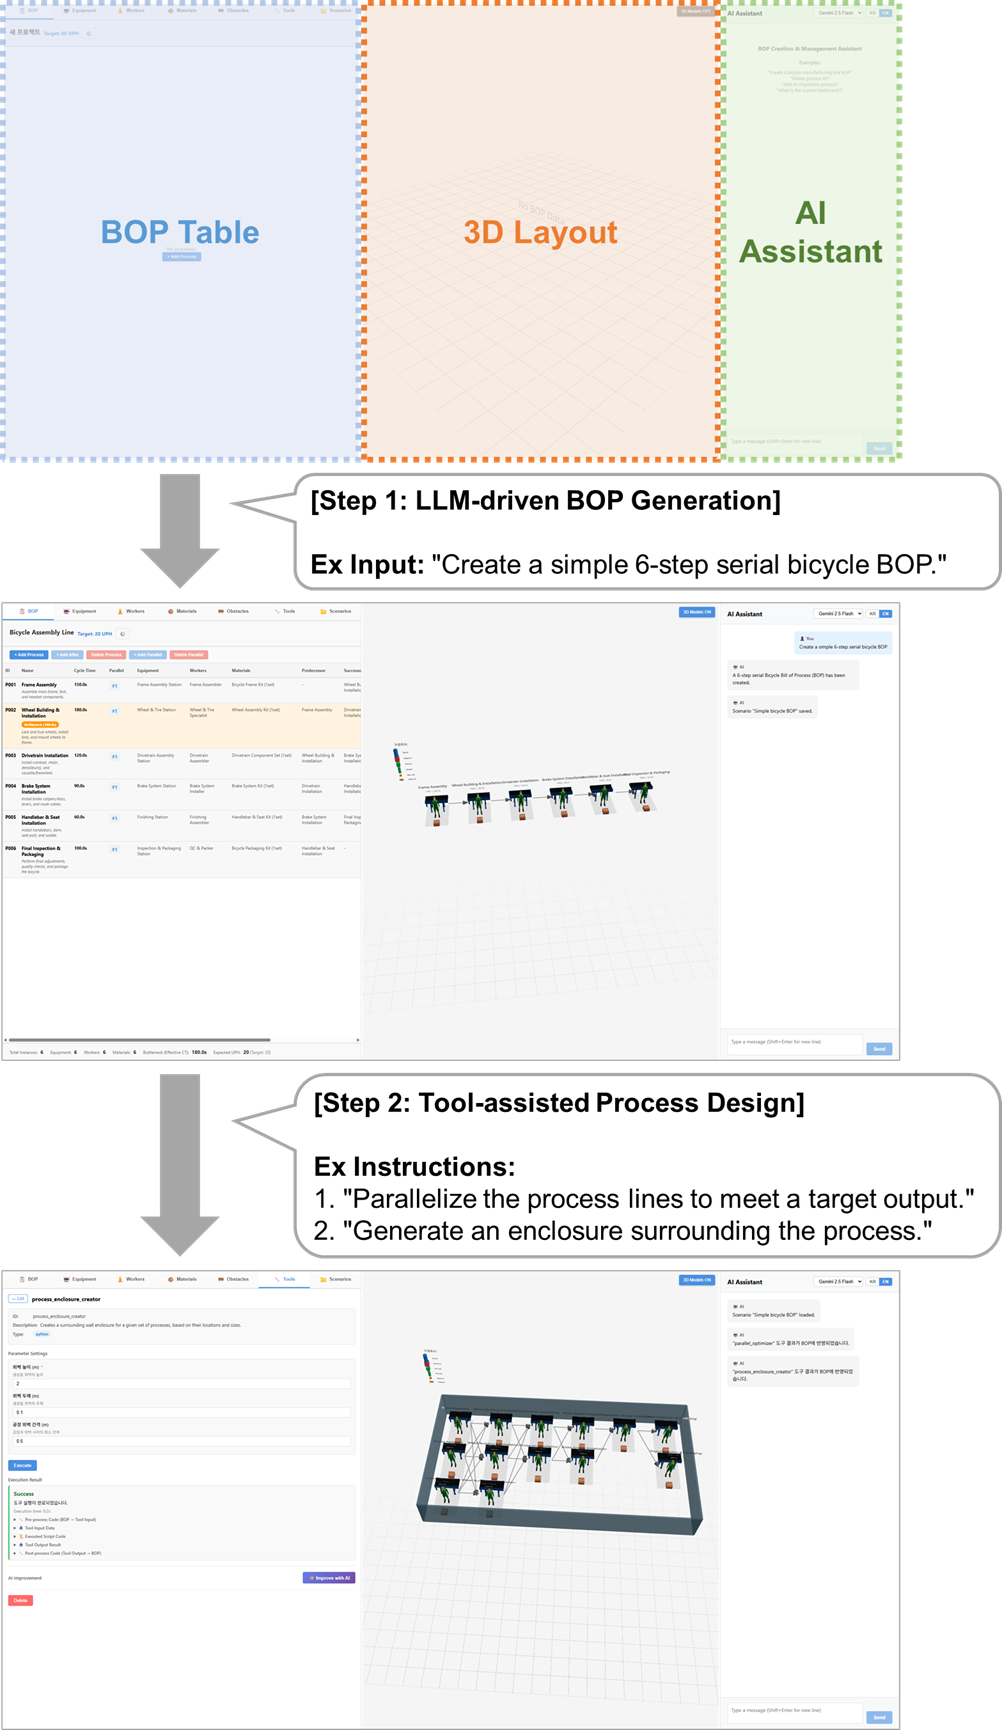
\includegraphics[width=\columnwidth]{fig1.png}
\caption{GDP system overview. Top: Integrated interface comprising BOP Table, 3D Layout, and AI Assistant. Step~1: LLM-based BOP generation. Step~2: Design refinement through external tool integration and Auto-Repair.}
\label{fig:overview}
\end{figure}

\subsection{LLM-Based BOP Generation (Step~1)}

Step~1 in Fig.~\ref{fig:overview} illustrates the process of generating simulation-ready process designs from natural language. For example, when a user inputs ``\textit{Create a simple 6-step serial bicycle BOP},'' the system automatically executes the following pipeline.

First, the user's request is classified into three types---new generation, existing modification, or simple query---and the corresponding prompt template is constructed. The prompt specifies manufacturing domain constraints alongside the output schema, including process count range (3--6), resource allocation rules (1--3 equipment, 1--2 workers, 1--3 materials per process), and cycle time range (10--300 seconds), confining LLM output to realistic bounds.

The JSON returned by the LLM undergoes three-stage validation: schema conformance, referential integrity (whether all resource IDs exist in the master lists), and DAG acyclicity (whether the process flow contains no cycles). Upon validation failure, the LLM is asked to regenerate, ensuring structural consistency.

For validated BOPs, automatic layout based on topological sorting places processes along the $X$-axis from predecessors, with parallel processes center-aligned along the $Z$-axis, immediately populating the BOP table and 3D view. When the user requests modifications via chat, a modification prompt including the current BOP as context is constructed and the same validation--layout--rendering pipeline repeats, preserving existing coordinates and resource configurations.

\subsection{Tool Integration and Auto-Repair (Step~2)}

Step~2 in Fig.~\ref{fig:overview} illustrates the process of refining the generated BOP through integration with external analysis tools. GDP provides three integration modes depending on the expert's proficiency and tool type, unified into a pluggable tool system with runtime registration.

\textbf{Mode~A: Existing Script Adapter Auto-Generation.}
When an expert uploads an existing analysis script (e.g., Python), the LLM analyzes the source code to automatically extract input/output schemas and user parameters. The LLM then generates two transformation functions: (i)~a preprocessor that converts the BOP to the input format expected by the tool, and (ii)~a postprocessor that interprets the tool's output and reflects it back into the BOP. This adapter code is executed within a whitelist-based sandbox to ensure security. This mode is suited for reusing existing assets while eliminating only the interface development burden.

\textbf{Mode~B: AI-Based Tool Logic Synthesis.}
When a tool's purpose and requirements are described in natural language without an existing analysis script, the LLM synthesizes complete tool code including the analysis logic itself. For example, a request such as ``find bottleneck processes and sort them by cycle time'' generates an analysis function that traverses BOP data and identifies bottlenecks. This mode enables experts without programming skills to immediately implement their domain knowledge as tools.

\textbf{Mode~C: Schema-Guided Optimization.}
When a predefined tool schema (input format, output format, parameter specification) is registered, the LLM references the schema to generate adapters with maximized mapping accuracy between BOP data and the tool. This mode supports workflows in enterprise environments requiring standardized interfaces, where tool development teams define only the schema and integration code is automatically generated.

\textbf{Tool Execution.}
Users configure tool-specific parameters and the system sequentially performs: (1)~preprocessor converts BOP to tool input, (2)~tool script execution, and (3)~postprocessor reflects results into BOP. Results are immediately rendered in the 3D view, and users can review and approve or cancel the changes.

\textbf{Auto-Repair Loop.}
When a runtime error occurs in the adapter during tool execution, the system automatically classifies the error type (environment constraint violation, type mismatch, etc.), and sends the adapter code along with error diagnostic information to the LLM to generate a corrected adapter. Re-execution is attempted with the corrected code, and this loop repeats up to $k$ times. The entire process is recorded in execution logs with timestamps, error diagnostics, and repair history to ensure traceability.

%% ============================================================
\section{Experiments and Results}
%% ============================================================

\subsection{Experiment 1: Zero-Shot Process Generation Performance}

For 10 heterogeneous manufacturing product families, we constructed a Ground Truth (GT) BOP dataset (83 process steps in total) directly extracted from publicly accessible HTML references, and evaluated the zero-shot process generation performance of four state-of-the-art LLMs. The GT dataset comprises EV battery cell (14 steps), automotive body-in-white BIW (9 steps), smartphone SMT (7 steps), semiconductor back-end (9 steps), solar PV module (9 steps), EV hairpin motor (8 steps), OLED display (6 steps), household washing machine (8 steps), continuous pharmaceutical tablet (6 steps), and tire (7 steps). All GT steps are directly quotable from reference sources. All models were tested under the same system prompt and temperature 0.0 conditions.

The granularity level of LLM-generated process steps may differ from the GT. For example, the LLM may decompose a single GT step ``Mixing'' into two steps ``Anode slurry mixing'' and ``Cathode slurry mixing,'' or conversely merge two GT steps into one. To fairly account for such granularity mismatches, we adopt \textbf{N:M coverage-based matching} instead of conventional 1:1 greedy matching. Step similarity is computed as a weighted average of the Jaccard coefficient and SequenceMatcher, with a threshold of 0.4 for match determination.

The evaluation metrics are as follows:
\begin{itemize}
\item \textbf{Recall}: Proportion of GT steps matched by at least one generated step. Measures GT coverage.
\item \textbf{Precision}: Proportion of generated steps matched to at least one GT step. Penalizes excessive decomposition or out-of-scope step generation.
\item \textbf{F1}: Harmonic mean of Precision and Recall.
\item \textbf{Sequence Consistency}: Degree to which the ordering of matched step pairs agrees with the GT ordering.
\end{itemize}

%% --- TABLE I ---
\begin{table*}[!t]
\caption{Average Performance by Model (N:M Coverage Matching)}
\label{tab:model_performance}
\centering
\begin{tabular}{l c c c c c c}
\hline
\textbf{Model} & \textbf{Recall} & \textbf{Precision} & \textbf{F1} & \textbf{Seq.\ Cons.} & \textbf{Avg.\ Steps} & \textbf{Latency (s)} \\
\hline
Gemini 2.5 Flash & 91.5\% & \textbf{93.1\%} & \textbf{92.1\%} & 65.6\% & 8.7 & \textbf{31.8} \\
GPT-5 Mini & \textbf{92.2\%} & 83.3\% & 87.1\% & 68.8\% & 10.4 & 120.9 \\
Gemini 2.5 Pro & 87.6\% & 88.4\% & 87.4\% & \textbf{80.3\%} & 9.2 & 53.4 \\
\hline
\textbf{3-Model Average} & \textbf{90.4\%} & \textbf{88.3\%} & \textbf{88.9\%} & \textbf{71.6\%} & \textbf{9.4} & \textbf{68.7} \\
\hline
GPT-5.2 & 64.1\% & 49.3\% & 54.9\% & 78.5\% & 12.0 & 69.9 \\
\hline
\end{tabular}
\end{table*}

The three models (Flash, Mini, Pro) achieved an average F1 of 88.9\% under N:M matching. Gemini 2.5 Flash achieved the highest F1 of 92.1\% with Precision 93.1\%, indicating the fewest unnecessary step generations. GPT-5 Mini achieved the highest Recall of 92.2\% but generated an average of 10.4 steps, resulting in a lower Precision of 83.3\%. Gemini 2.5 Pro excelled in Sequence Consistency at 80.3\%. By product, all three models achieved 100\% Recall on P07 (OLED) and P10 (Tire), while P02 (Automotive BIW, 70.4\%) was lowest due to stamping and welding operating as separate plant units. In cost-performance terms, Flash achieved F1 92.1\% with the lowest latency of 31.8 seconds, making it optimal for real-time prototyping.

\textbf{Over-Decomposition Analysis of Large Models (GPT-5.2).}
GPT-5.2 recorded an F1 of only 54.9\%, significantly lower than the three models. Switching from 1:1 greedy matching (F1 43.6\%) to N:M matching improved F1 by 11.3pp, confirming underestimation due to granularity mismatches. Notably, P04 (Semiconductor, +22.2pp) and P05 (Solar PV, +33.3pp) showed large improvements, while P02 (Automotive BIW) and P09 (Pharma) showed no improvement due to core process omissions. GPT-5.2 generated an average of 12.0 steps (+44.6\% relative to the GT average of 8.3), suggesting that large models tend to excessively incorporate shop-floor-level detailed knowledge.

\subsection{Experiment 2: Automatic Adapter Generation and Auto-Repair Robustness}

To evaluate the performance of GDP's schema-based automatic adapter synthesis and Auto-Repair mechanism, we designed 10 analysis tools of varying difficulty and 8 BOP scenarios with diverse structures, scales, and domains (2--14 processes, linear/parallel/DAG structures), conducting a total of 320 execution experiments (10 tools $\times$ 8 BOPs $\times$ 4 $k$ values). Gemini 2.5 Flash was used as the adapter generation model, and the repair budget $k$ was varied from 0 (baseline, no repair) to 3, with two tiers of evaluation: (1)~Execution Pass Rate---whether the adapter completes without errors, and (2)~Output Correctness---whether the tool's output satisfies domain invariant conditions.

The 10 tools were classified into three difficulty levels based on the complexity of BOP-to-tool data transformation: Easy (2 tools, simple field extraction), Medium (5 tools, multi-array cross-referencing or coordinate transformation), and Hard (3 tools, complex graph transformation or multi-step reasoning). Output correctness was measured using domain-specific property-based validators designed for each tool, checking mathematical consistency (e.g., whether the bottleneck process has the maximum effective cycle time), structural integrity (e.g., non-negative layout coordinates), and aggregation accuracy (e.g., distribution sum matching totals).

\subsubsection{Execution Pass Rate Analysis}

TABLE~\ref{tab:pass_rate} shows the execution pass rate by repair budget $k$.

%% --- TABLE IV ---
\begin{table}[!t]
\caption{Execution Pass Rate by Repair Budget $k$}
\label{tab:pass_rate}
\centering
\begin{tabular}{c c c c}
\hline
$k$ & \textbf{Pass} & \textbf{Fail} & \textbf{Pass Rate} \\
\hline
0 & 64 & 16 & 80.0\% \\
1 & 79 & 1  & 98.8\% \\
2 & 80 & 0  & \textbf{100.0\%} \\
3 & 80 & 0  & \textbf{100.0\%} \\
\hline
\end{tabular}
\end{table}

At baseline ($k{=}0$), LLM-generated adapters exhibited an execution pass rate of 80.0\% (64/80), with two failure modes observed across two tools. Easy tools (2) achieved 100\% at all $k$ values, while among Medium tools (5), \texttt{worker\_skill\_matcher} raised a TypeError during the postprocessing phase. Hard tools (3) showed a pass rate of 66.7\% (16/24), with \texttt{layout\_compactor} raising an ImportError due to a forbidden \texttt{copy} module import in the sandbox, while \texttt{energy\_estimator} and \texttt{takt\_time\_optimizer} passed at baseline.

Activating Auto-Repair at $k{=}1$ raises the pass rate to 98.8\% (79/80), reaching 100\% at $k{=}2$. Of the 47 total repair events, 93.6\% succeeded in a single attempt, with an average of 1.06 repair attempts, demonstrating rapid convergence. This is because error messages provide explicit diagnostic information for environment constraint violations (ImportError) and schema mapping errors (TypeError), effectively guiding the LLM's self-correction.

\subsubsection{Output Correctness --- Two-Tier Evaluation}

Execution pass alone cannot fully evaluate adapter quality. Even in a 3D digital twin, error-free execution may result in walls or equipment rendered at incorrect positions, or optimization results that are logically contradictory. TABLE~\ref{tab:two_tier} compares execution pass rate and output correctness in a two-tier evaluation.

%% --- TABLE V ---
\begin{table}[!t]
\caption{Two-Tier Evaluation --- Execution Pass Rate vs.\ Output Correctness}
\label{tab:two_tier}
\centering
\begin{tabular}{c c c c}
\hline
$k$ & \textbf{Exec.\ Pass} & \textbf{Output Corr.} & \textbf{Full Pass} \\
\hline
0 & 80.0\%  & 98.4\% (63/64)  & 78.8\% \\
1 & 98.8\%  & 84.8\% (67/79)  & 83.8\% \\
2 & 100.0\% & 83.8\% (67/80)  & \textbf{83.8\%} \\
3 & 100.0\% & 83.8\% (67/80)  & \textbf{83.8\%} \\
\hline
\end{tabular}
\end{table}

At $k{=}2$, the execution pass rate reaches 100\%, but only 83.8\% of outputs satisfy all invariant conditions. That is, \textbf{16.2\% of adapters execute without errors but produce semantically incorrect results}---a failure type undetectable by execution-only evaluation.

TABLE~\ref{tab:tool_accuracy} shows per-tool output correctness. Seven tools (all Easy + 4 Medium + 1 Hard) achieved 100\% output correctness, while semantic errors were observed in three tools.

%% --- TABLE VI ---
\begin{table*}[!t]
\caption{Per-Tool Output Correctness (Among Execution Passes, $k{=}2$)}
\label{tab:tool_accuracy}
\centering
\begin{tabular}{l c c c l}
\hline
\textbf{Tool} & \textbf{Difficulty} & \textbf{Accuracy} & \textbf{Avg.\ Score} & \textbf{Primary Error} \\
\hline
bottleneck\_analyzer       & E & 100\% & 100.0\% & --- \\
line\_balance\_calculator  & E & 100\% & 100.0\% & --- \\
equipment\_utilization     & M & 100\% & 100.0\% & --- \\
material\_flow\_analyzer   & M & 100\% & 100.0\% & --- \\
process\_distance\_analyzer & M & 100\% & 100.0\% & --- \\
safety\_zone\_checker      & M & 100\% & 100.0\% & --- \\
worker\_skill\_matcher     & M & \textbf{12\%} & 95.1\% & Distribution sum mismatch \\
energy\_estimator          & H & 100\% & 100.0\% & --- \\
layout\_compactor          & H & \textbf{39\%} & 95.2\% & Negative coords, span expansion \\
takt\_time\_optimizer      & H & \textbf{88\%} & 99.7\% & Parallel count decrease \\
\hline
\end{tabular}
\end{table*}

\texttt{layout\_compactor} (Hard, 39\% accuracy) generated negative coordinates (e.g., $z = -4.0$) or expanded the layout span instead of compacting it, manifesting as walls and equipment rendered at incorrect positions in the 3D digital twin. \texttt{worker\_skill\_matcher} (Medium, 12\% accuracy) produced a \texttt{skill\_distribution} field inconsistent with the \texttt{matches} array, omitting some workers from the distribution summary. \texttt{takt\_time\_optimizer} (Hard, 88\% accuracy) incorrectly reduced a process's parallel count from 2 to 1 on a large-scale BOP (14 processes), violating optimization constraints.

These results demonstrate that \textbf{Auto-Repair effectively resolves execution errors but does not guarantee semantic correctness}. A tendency toward degraded output correctness with increasing tool complexity was observed, suggesting that more complex BOP-to-tool data transformations make it harder for the LLM to generate accurate mappings. From a practical standpoint, a two-tier quality assurance framework that complements Auto-Repair with runtime property-based validation is needed to ensure not only executability but also domain correctness.

\subsection{Experiment 3: Design Task Efficiency Evaluation}

To evaluate the practical effectiveness of GDP, we measured design time with five engineers with 3--15 years of experience in automotive, semiconductor, and display process design. Regarding scenario design, existing standards such as ISO 23247~\cite{b3} do not provide publicly available standard production line specifications for benchmarking purposes. We therefore designed a mock scenario that reflects real-world manufacturing characteristics (mixed manual/automated operations, diverse resource types, and the presence of bottlenecks). The scenario is a ``High-end E-Bike Assembly Simulation Line'' with a 6-process serial structure (Frame Loading 20s, Drive Unit Assembly 30s, Battery \& Wiring 45s, Wheel Set Integration 25s, Steering \& Brake Setting 40s, Final Inspection 20s) and a target UPH of 100.

Each participant performed two conditions sequentially:
\begin{itemize}
\item \textbf{CASE~A (Manual Design)}: Manually construct the process table, resource assignments, and 3D layout using only GDP's editing functions.
\item \textbf{CASE~B (AI-Assisted Design)}: Input natural language specifications into the GDP AI Assistant to automatically generate the BOP and integrate analysis tools.
\end{itemize}

The task consists of two phases. In \textit{Task~1 (Initial Setup)}, participants generate a 6-process serial BOP from the specification table and arrange resources and the layout. In \textit{Task~2 (Line Optimization)}, participants (1)~analyze the current line's UPH and parallelize the bottleneck process (Battery \& Wiring, 45s) to meet the target UPH of 100, and (2)~generate an enclosure surrounding the entire line to secure the safety zone.

%% --- TABLE: Experiment 3 results (to be filled after experiment) ---
\begin{table}[!t]
\caption{Design time comparison by condition}
\label{tab:design_time}
\centering
\begin{tabular}{l c c c}
\hline
\textbf{Condition} & \textbf{Mean (min)} & \textbf{SD} & \textbf{Reduction} \\
\hline
CASE~A (Manual) & OO.O & OO.O & --- \\
CASE~B (AI-Assisted) & OO.O & O.O & OO.O\% \\
\hline
\end{tabular}
\end{table}

%% TODO: Update TABLE~\ref{tab:design_time} and narrative below after collecting results
CASE~A averaged OO.O~min (SD OO.O) and CASE~B averaged OO.O~min (SD O.O), yielding an average time reduction of OO.O\% with AI-assisted design over manual design. The largest time savings were observed in Task~1 (initial BOP construction), where a single natural language sentence generated all six processes with resource assignments. In Task~2 (line optimization), bottleneck analysis tool integration and automatic enclosure generation proved more efficient than manual manipulation.

%% ============================================================
\section{Conclusion}
%% ============================================================

This study proposes the GDP framework, which leverages LLMs to remove barriers in manufacturing process design and tool integration. GDP accelerates digital twin prototyping through zero-shot process design for non-experts and three tool integration modes for experts, with a Process-centric flattened data model referencing the Siemens BOP concept that simultaneously achieves token efficiency and generation accuracy.

Experimental results show that three LLMs achieved an average F1 of 88.9\% (Recall 90.4\%, Precision 88.3\%) for zero-shot process generation across 10 manufacturing products under N:M coverage matching. Additional analysis reveals that the large model (GPT-5.2) over-decomposed processes, resulting in an F1 of only 54.9\%, but the introduction of N:M matching confirmed a fair evaluation improvement of 11.3pp over 1:1 matching (43.6\%).

In the tool integration experiment (10 tools $\times$ 8 BOPs $\times$ 4 conditions = 320 runs), the Auto-Repair mechanism improved the baseline execution pass rate of 80.0\% to 100\% with at most two repairs (average 1.06 attempts). Furthermore, by introducing a two-tier evaluation (execution pass + output correctness) with property-based validation, we discovered that 16.2\% of adapters constitute ``silent failures''---executing successfully but producing semantically incorrect results. This implies that while Auto-Repair is effective at resolving execution errors, it does not guarantee domain correctness, and supplementation with runtime property validation is necessary. An evaluation with five process design experts confirmed significant time reduction when using GDP features over manual design. Furthermore, the diverse mock production line data generated by GDP holds potential as a testbed for Physical AI and humanoid robots to pre-train on manufacturing tasks in virtual environments~\cite{b15}.

However, GDP's current data model lacks detailed specification data in the master tables (equipment, workers, materials)---such as rated power, available operating hours, and maintenance cycles for equipment; shift conditions and fatigue constraints for workers; and supply lead times and inventory constraints for materials. The absence of such detailed data limits the ability of advanced analysis tools (e.g., line balancing, energy optimization) to perform precise optimization reflecting realistic constraints.

Future work includes (1)~extending the master table schema to accommodate detailed constraints for equipment, workers, and materials (utilization rates, shift patterns, supply lead times, etc.) and thereby improving the optimization precision of analysis tools, (2)~improving semantic accuracy through a secondary repair loop (validation-driven repair) that uses output validation results as feedback, and (3)~developing automated pipelines for constructing virtual manufacturing environments for Physical AI training. Ultimately, we aim for this research to serve as foundational work for standardized process data generation and tool integration in conjunction with digital twin standard frameworks such as ISO 23247.

%% ============================================================
\section*{Acknowledgment}
%% ============================================================

%% TODO: Write acknowledgments

%% ============================================================
\begin{thebibliography}{00}
\bibitem{b1} M.~Grieves and J.~Vickers, ``Digital twin: Mitigating unpredictable, undesirable emergent behavior in complex systems,'' in \textit{Transdisciplinary Perspectives on Complex Systems}, Springer, 2017, pp.~85--113.
\bibitem{b2} F.~Tao, J.~Cheng, Q.~Qi, M.~Zhang, H.~Zhang, and F.~Sui, ``Digital twin-driven product design, manufacturing and service with big data,'' \textit{Int.\ J.\ Adv.\ Manuf.\ Technol.}, vol.~94, pp.~3563--3576, 2018.
\bibitem{b3} ISO 23247-1:2021, ``Automation systems and integration --- Digital twin framework for manufacturing --- Part 1: Overview and general principles,'' 2021.
\bibitem{b4} T.~H.~J.~Uhlemann, C.~Lehmann, and R.~Steinhilper, ``The digital twin: Realizing the cyber-physical production system for Industry 4.0,'' \textit{Procedia CIRP}, vol.~61, pp.~335--340, 2017.
\bibitem{b5} F.~Ji, F.~Ocker, M.~Zou, B.~Vogel-Heuser, and M.~Oligschlager, ``Identifying inconsistencies in the design of large-scale casting systems --- An ontology-based approach,'' in \textit{Proc.\ IEEE Int.\ Conf.\ Autom.\ Sci.\ Eng.\ (CASE)}, 2022, pp.~319--325.
\bibitem{b6} T.~Brown \textit{et al.}, ``Language models are few-shot learners,'' in \textit{Proc.\ Advances in Neural Inform.\ Process.\ Syst.\ (NeurIPS)}, 2020, pp.~1877--1901.
\bibitem{b7} Siemens Digital Industries Software, ``Bill of process,'' 2023. [Online]. Available: \url{https://www.sw.siemens.com/en-US/technology/bill-of-process/}
\bibitem{b8} Y.~Xia, Z.~Xiao, N.~Jazdi, and M.~Weyrich, ``Generation of asset administration shell with large language model agents: Toward semantic interoperability in digital twins in the context of Industry 4.0,'' \textit{IEEE Access}, vol.~12, pp.~84863--84877, 2024.
\bibitem{b9} Q.~Xu, G.~Zhou, C.~Zhang, F.~Chang, Y.~Cao, and D.~Zhao, ``Generative AI and DT integrated intelligent process planning: A conceptual framework,'' \textit{Int.\ J.\ Adv.\ Manuf.\ Technol.}, vol.~133, no.~5--6, pp.~2461--2485, 2024.
\bibitem{b10} W.~Kritzinger, M.~Karner, G.~Traar, J.~Henjes, and W.~Sihn, ``Digital Twin in manufacturing: A categorical literature review and classification,'' \textit{IFAC-PapersOnLine}, vol.~51, no.~11, pp.~1016--1022, 2018.
\bibitem{b11} AutomationML, ``IEC 62714: Engineering data exchange format for use in industrial automation systems engineering,'' 2018.
\bibitem{b12} M.~Chen \textit{et al.}, ``Evaluating large language models trained on code,'' \textit{arXiv preprint arXiv:2107.03374}, 2021.
\bibitem{b13} X.~Chen, M.~Lin, N.~Sch\"arli, and D.~Zhou, ``Teaching large language models to self-debug,'' in \textit{Proc.\ Int.\ Conf.\ Learn.\ Representations (ICLR)}, 2024.
\bibitem{b14} Y.~Brun \textit{et al.}, ``Engineering self-adaptive systems through feedback loops,'' in \textit{Software Engineering for Self-Adaptive Systems}, Springer, 2009, pp.~48--70.
\bibitem{b15} J.~Tobin, R.~Fong, A.~Ray, J.~Schneider, W.~Zaremba, and P.~Abbeel, ``Domain randomization for transferring deep neural networks from simulation to the real world,'' in \textit{Proc.\ IEEE/RSJ Int.\ Conf.\ Intell.\ Robots Syst.\ (IROS)}, 2017, pp.~23--30.
\end{thebibliography}

\end{document}
